% Chapter Template

\chapter{System design} % Main chapter title

\label{Chapter3} % Change X to a consecutive number; for referencing this chapter elsewhere, use \ref{ChapterX}
I kljdf kljdf lke dakd .
kladf.

%----------------------------------------------------------------------------------------
%	SECTION 1
%----------------------------------------------------------------------------------------

\section{Overview}

Range based localization systems are depending on an infrastructure in the area of the localization:
\begin{itemize} 
\item \textbf{Target Node (TAG)} which is the device that is localized. 
\item \textbf{Anchor Nodes (AN)}that are placed on carefully chosen points in the building, to encounter the best coverage of the whole area.
\end{itemize}

\begin{figure}[th]
\centering
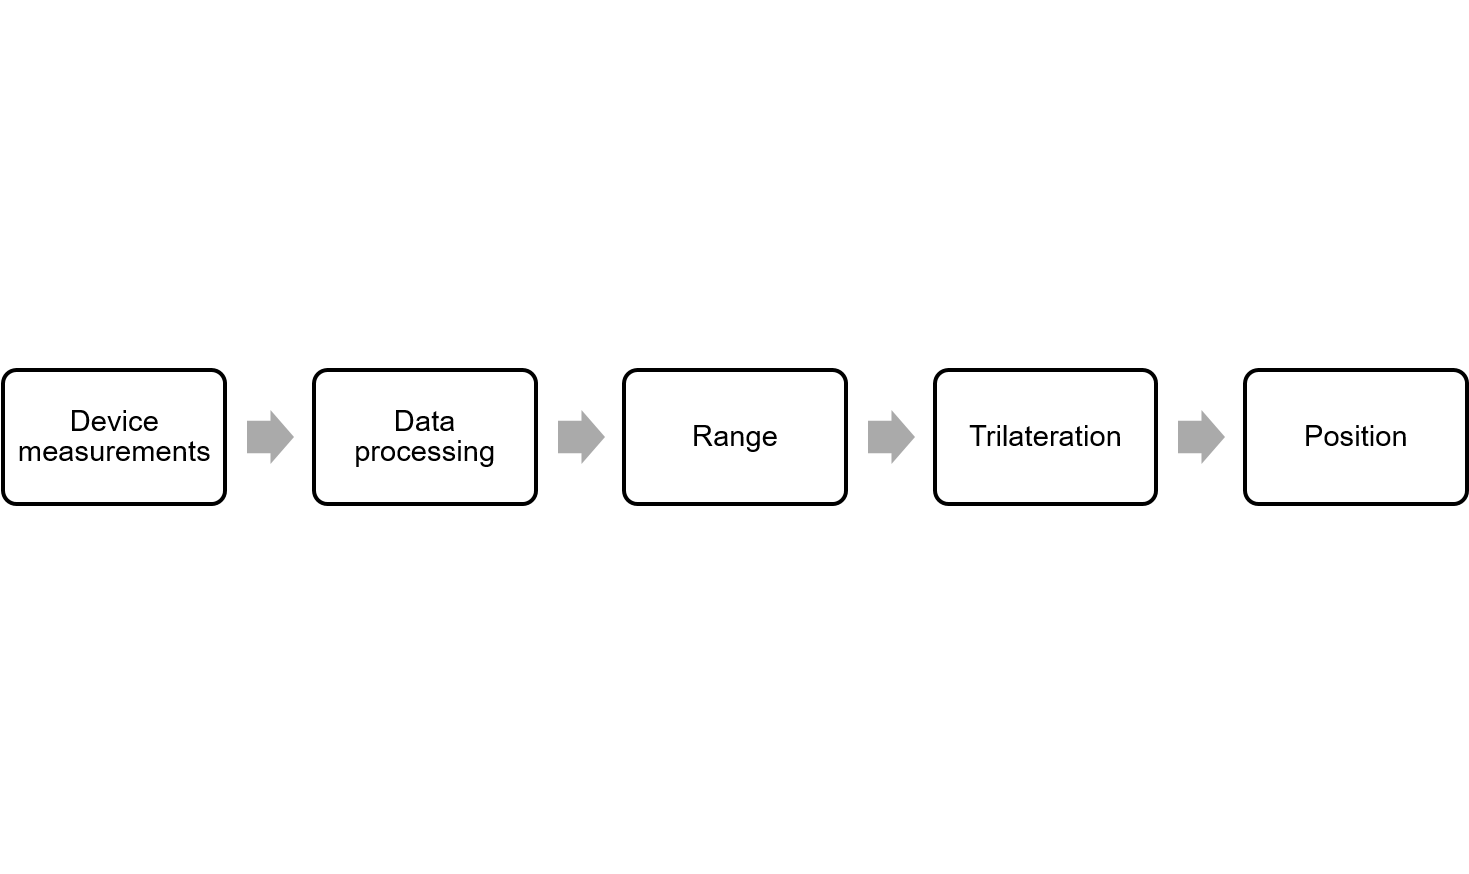
\includegraphics[width=1.0\textwidth]{Figures/ranging_process1}
\decoRule
\caption[Ranging process1]{A simple ranging process.}
\label{fig:ranging_process1}
\end{figure}

As shown in figure \ref{fig:ranging_process1}, a simplified localization system work as follows:
Either the TAG, the anchor or both of them collect data used for localization. The data can be a signal strength, a round trip time or IMU measurement.
In a processing unit - on the TAG or on a seperate server - the data is processed and converted into a distance. This is repeated for every anchor node.
The last step contains trilateration of the position using the ranges of every AN to the TAG.

In this abridged scenario, some difficulties are left out. Full indoor localization systems are more complex, as they use ingenious algorithms to improve the accuracy of the estimated ranges or improve the system by adding weighting to deal with incorrect range measures.


%----------------------------------------------------------------------------------------
%	SECTION 2
%----------------------------------------------------------------------------------------

\section{Setup}

Sed ullamcorper quam eu nisl interdum at interdum enim egestas. Aliquam placerat justo sed lectus lobortis ut porta nisl porttitor. Vestibulum mi dolor, lacinia molestie gravida at, tempus vitae ligula. Donec eget quam sapien, in viverra eros. Donec pellentesque justo a massa fringilla non vestibulum metus vestibulum. Vestibulum in orci quis felis tempor lacinia. Vivamus ornare ultrices facilisis. Ut hendrerit volutpat vulputate. Morbi condimentum venenatis augue, id porta ipsum vulputate in. Curabitur luctus tempus justo. Vestibulum risus lectus, adipiscing nec condimentum quis, condimentum nec nisl. Aliquam dictum sagittis velit sed iaculis. Morbi tristique augue sit amet nulla pulvinar id facilisis ligula mollis. Nam elit libero, tincidunt ut aliquam at, molestie in quam. Aenean rhoncus vehicula hendrerit.

%----------------------------------------------------------------------------------------
%	SECTION 3
%----------------------------------------------------------------------------------------

\section{Algorithms}

Sed ullamcorper quam eu nisl interdum at interdum enim egestas. Aliquam placerat justo sed lectus lobortis ut porta nisl porttitor. Vestibulum mi dolor, lacinia molestie gravida at, tempus vitae ligula. Donec eget quam sapien, in viverra eros. Donec pellentesque justo a massa fringilla non vestibulum metus vestibulum. Vestibulum in orci quis felis tempor lacinia. Vivamus ornare ultrices facilisis. Ut hendrerit volutpat vulputate. Morbi condimentum venenatis augue, id porta ipsum vulputate in. Curabitur luctus tempus justo. Vestibulum risus lectus, adipiscing nec condimentum quis, condimentum nec nisl. Aliquam dictum sagittis velit sed iaculis. Morbi tristique augue sit amet nulla pulvinar id facilisis ligula mollis. Nam elit libero, tincidunt ut aliquam at, molestie in quam. Aenean rhoncus vehicula hendrerit.